\documentclass[12pt, letterpaper]{article}

\usepackage[margin=1in]{geometry}
\usepackage[tiny]{titlesec}
\usepackage[section]{placeins}
\usepackage{indentfirst, setspace}
\usepackage{amsmath,amsthm,amsfonts,amssymb,amscd}
\usepackage{booktabs,subcaption}
\usepackage{enumerate}
\usepackage{fancyhdr}
\usepackage{mathrsfs}
\usepackage{xcolor}
\usepackage{graphicx}
\usepackage{listings}
\usepackage{txfonts}
\usepackage{siunitx}
\usepackage{apacite}
% \usepackage{float}
\doublespacing
\setlength{\parindent}{4em}
\graphicspath{{./images/}}

\begin{document}


\title{\vspace{-2.0cm}Analyzing the Spread of Memes with Epidemiological Models}
\author{Kavin Nguyen \\ AMATH 383, University of Washington}
\date{March 12, 2020}
\maketitle

\begin{abstract}
Memes are elements of culture that have the potential to spread rapidly across the internet. Modeling how these memes propagate over time opens the door for interested parties to maximize the popularity and lifespan of memes in order to leverage them for political, financial, or other personal gain. This paper analyzes the claim that memes spread virally by fitting the SIR model, a model commonly discussed in epidemiological contexts, to real-world time series data on the popularity of internet memes. Analysis were performed on 6 memes with interest data on each meme acquired by Google Trends. The temporal dynamics of diseases were found to translate remarkably well to memes, indicating that memes are infectious in nature in a way similar to viruses. 
\end{abstract}

%% main text
\section*{Introduction}

Evolutionary biologist Richard Dawkins coined the term “meme” to mean a piece of culture that undergoes transmission in a way that is analogous to genetic transmission, and can change over time in a way that is analogous to biological evolution. \cite{dawkins_1989} This term “piece of culture” is intentionally vague as it encompasses everything that can carry ideas within a culture much like how genes carry genetic information. Proponents of memetics, the study of information based on models for Darwinian evolution, argue that memes undergo self-replication, mutation, and natural selection similarly to genes in a biological context. The legitimacy of memetics is debated, with critics arguing that most of the assertions relating memes and genes are unsupported or incorrect. This paper will support a possible model for the spread of memes, but will not be evaluating how they evolve over time.

The concept being explored is that ideas, behaviors, and other identity-influencing material are stored in the brain and spread through memes like how genetic code can be spread by viruses. This parallel between the spread of culture through memes and the spread of disease through viruses is widely recognized in society. Videos, images, trends, movements, and products that gain popularity quickly are said to be viral in nature. Companies try to engage in "viral marketing" by attempting to sell their products with the aid of social media. Those who engage with a meme have the ability to metaphorically sneeze those memes into the face of others through the multitude of social media platforms available today. Twitter, YouTube, Facebook, Instagram, Reddit, 4chan, and recently TikTok have all given users the ability to spread their cultural influence to “susceptibles”, those who have not yet experienced their meme. If they engage with the meme, they become “infected”, and may propagate the meme through the aforementioned channels. Once they have grown tired of the meme, they will be considered “recovered”, and will no longer promote the meme (at least until the meme has sufficiently mutated in a way as to become novel once again). This process may bring to mind the popular epidemiological model known as the SIR model.

The SIR model \cite{kermack1927contribution} is a set of differential equations where the solutions $S(t)$, $I(t)$, and $R(t)$ describe the number of people who are susceptible to a disease, are infected with the disease, and have recovered from the disease, respectively. This model assumes that the population remains constant, and it is a reasonable assumption in the context of internet memes as the number of people who newly engage with memes and the number of people who no longer engage with them should not change much over the few months that a particular meme is relevant. This model also assumes that those who are considered “recovered” can no longer infect others.

Google provides a useful tool when it comes to analyzing internet trends. This tool, fittingly named Google Trends, gives data about the popularity of search terms since 2004. It is assumed that the popularity of a meme is proportional to the number of people who search for the meme on Google. Google Trends serves time series data where the peak amount of searches involving a term of interest is normalized to a value of 100. A significant disadvantage of this tool is that it does not give insight into how popular a particular meme was compared to other memes. It does not provide a sense of the absolute number of searches for a particular term. This makes it hard to draw connections across different memes, but it does not prevent a epidemiological model from being used to describe the growth and decline of a particular meme.

This paper examines how well the spread of 6 of the most popular memes of the past year in the United States (judged by qualitative observation on my part) fit a model used to describe the spread of viruses. The name of each meme used in the Google Trends search are: "surprised pikachu", "me and the boys", "area 51", "ok boomer", "yelling at cat", and "baby yoda". Searching for these online or with \textit{knowyourmeme.com} will yield explanations, origins and examples for the meme, so neither background for these memes nor images of them will be provided here.

There is existing work examining the spread of cultural phenomena using epidemic models. \cite{bauckhage2011insights} applies the SIRS model to the spread of memes using data collected from Google Insights (a service that has been merged with Google Trends as of 2012). The SIRS model is a slightly more complex model compared to the standard SIR model. It takes into account the possibility for recovered people to become susceptible again. Bauckhage (2011) applied their model to 150 memes and found that "SIRS models reproduces the general behavior of memes, but, in particular for memes that are characterized by bursty activities, tend to underestimate the early early contagious stages of the meme" \cite{bauckhage2011insights}. This means that memes that grow too quickly initially are modeled poorly by the SIRS model, but the decay of a meme's popularity is tracked well. Bauckhage (2011) then applied a log-normal distribution to model the popularity of memes and found that they fit much better than SIRS in more cases. He concludes that while the log-normal distribution better characterizes instances where the popularity of memes change rapidly, the SIRS model still gives a good account of the growth and decline of memes in general.

Another paper that found similar results using an epidemics model was \cite{wang2011epidemiological}. Wang and Wood (2011) used a modified version of the SIR model where recovered people can still become infected albeit at a lower rate than susceptible people. Specifically, the rate of infection increases as the number of infected and recovered people increases. Wang and Wood (2011) still considers this modified SIR model to be a model for infectious diseases, and concludes that their work indicates memes can be considered infectious in nature because their modified model "provides excellent fits for data sets exhibiting a sharp initial spike followed by a gradual taper" \cite{wang2011epidemiological}. They came to this conclusion by fitting the model to Google Trends data of 3 memes. Bauckhage (2011) and Wang (2011) came to similar conclusions using different models for infectious diseases, but Wang and Wood (2011) found that their model fits rapid growth and declines well while Bauckhage (2011) found that the SIRS model could not. This paper will examine how well the standard SIR model maps onto the spread of internet memes, and it will be used to justify (or disprove) the idea that memes spread virally.

\cite{leskovec2007dynamics}, a more well known paper compared to the previous two, looked at modeling viral marketing. While not exactly the same as the spread of memes, both leverage social networks and personal interaction in order to spread. Leskovec et. al (2007) examines how product recommendations influence purchases, and notes that epidemic models like SIR and SIRS assume that the entire population is equally susceptible to marketing as these models describe infections with 1 or 2 parameters. Leskovec et. al (2007) observes that contrary to the assumption that the probability of infection increases with increasing contact, as epidemic models make, the probability of infection actually decreases with repeated interaction in the case of viral marketing. They found that there are too many variables involved in social networks to be simply described by SIR type models, so because of this, they concluded that viral marking is in general not as epidemic as we think. These results are interesting, but memes are distinct enough from products that parallels between viral marketing and memes are to be taken with hesitation. For one, purchasing and endorsing a product requires more effort and commitment than sharing a meme, so memes may spread more virally than viral marketing.

The following section will give a formulation of the model. Then the model will be used to fit Google Trends data and explore implications of the results. Finally, the paper will end with a conclusion summarizing the results.

\section*{Model Formulation}
The standard SIR model is usually given as the following system of differential equations of $S(t)$, $I(t)$, and $R(t)$.
\begin{equation}
\begin{aligned}
\frac{dS}{dt} &= -\frac{\beta IS}{N}, \\
\frac{dI}{dt} &= \frac{\beta IS}{N} - \gamma I, \\
\frac{dR}{dt} &= \gamma I
\end{aligned}
\label{eq: logical 1}
\end{equation}

$\beta$ is the transmission rate proportionality constant, and it equals the average number of contacts sufficient for disease transmission. In this case, it represents the likelihood of someone becoming infected with the meme. $1/\gamma$ is the amount of time that a disease is infectious before the infected becomes recovered and can no longer infect others. It represents the amount of time before an infected loses interest in the meme.

Because the total population $N$ that can engage with a particular meme is assumed to be constant, $S(t) + I(t) + R(t) = N$, and $\frac{dS}{dt} + \frac{dI}{dt} + \frac{dR}{dt} = 0$. This is clearly seen in equations (1) where the rate of people entering the infected state is equal to the rate of people exiting the susceptible state, and the rate of people entering the recovered state is equal to the rate of people leaving the infected state. Another thing to note is that the some terms are divided by $N$. This is mainly because $I * S$ gives the units of $[people]^2$, so dividing by N maintains the unit of $[people]$.

The differential equations are subject to the following initial conditions:
\begin{equation}
\begin{aligned}
S(0) &= S_0 > 0 \\
I(0) &= 1 \\
R(0) &= 0 \\
\end{aligned}
\label{eq: logical 2}
\end{equation}

The first condition means that for any given meme, there is a fixed number of people who will become infected by that meme, and that number is greater than 0. The second condition implies that memes originate from the mind of a single person, who then spreads it around on social media. The last initial condition is obvious as there cannot be recovered people if no one but the creator has been infected. From these initial conditions, $N = S_0 - 1$.

The only solution of the three that will be plotted is $I(t)$ because it is what should correlate to the Google Trends data. In order to fit the number of infected as a function of time to the data, the equations (1) need be solved using the initial conditions (2). Varying the the constants $\beta$, $\gamma$, and $N$  will change the shape of $I(t)$. These are the parameters that will be used to optimize the fit to the data with the method of optimization being the method of non-linear least squares.



\section*{Results and Implications}
The optimized parameters from the results of the non-linear least square fit is given in Table 1. Fig. 1 shows the plots of $I(t)$ using the respective parameters from Table 1 on top of the data from Google Trends.

\begin{table*}[htbp!]
\centering
    \caption{Optimized SIR Parameters}
    \begin{tabular}{@{\extracolsep{1em}}lccc}
        \toprule
        Meme & N & $\beta$ & $\gamma$ \\
        \midrule
        surprised pikachu & 7.68e1 & 5.77e-1 & 2.08e-2\\
        me and the boys & 1.14e2 & 9.16e-2 & 5.06e-2 \\
        area 51 & 2.18e2 & 1.49 & 3.25e-1\\ 
        ok boomer & 7.69e1 & 6.38e-1 & 2.57e-2\\ 
        yelling at cat & 9.91e1 & 4.59e-1 & 5.33e-2\\
        baby yoda & 1.02e2 & 5.23e-1 & 1.00e-3\\
        \bottomrule
    \end{tabular}
\end{table*}

\begin{figure}[htbp!]
\begin{subfigure}{.5\textwidth}
    \centering
    \caption{"surprised pikachu" starting 28/10/2018}
    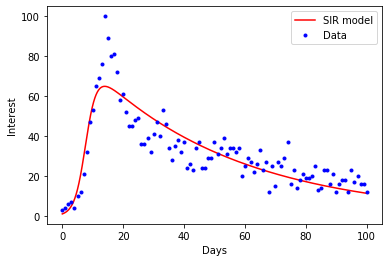
\includegraphics[width=0.8\linewidth]{pikachu}
    \label{fig:sfig1}
\end{subfigure}
\begin{subfigure}{.5\textwidth}
    \centering
    \caption{"me and the boys" starting 30/5/2019}
    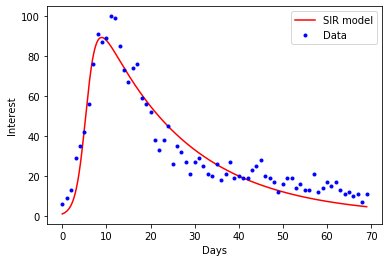
\includegraphics[width=0.8\linewidth]{boys}
    \label{fig:sfig2}
\end{subfigure}
\begin{subfigure}{.5\textwidth}
    \centering
    \caption{"area 51" starting 8/7/2019}
    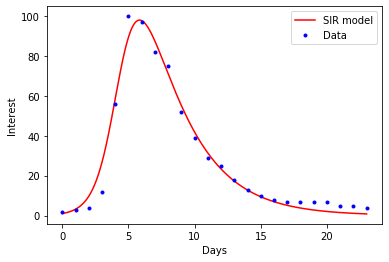
\includegraphics[width=0.8\linewidth]{area51}
    \label{fig:sfig1}
\end{subfigure}
\begin{subfigure}{.5\textwidth}
    \centering
    \caption{"ok boomer" starting 27/10/2019}
    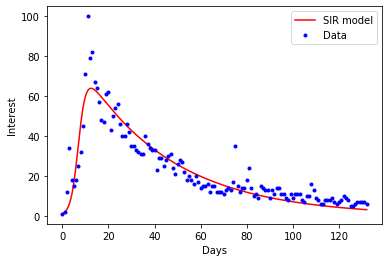
\includegraphics[width=0.8\linewidth]{boomer}
    \label{fig:sfig1}
\end{subfigure}
\begin{subfigure}{.5\textwidth}
    \centering
    \caption{"yelling at cat" starting 27/9/2019}
    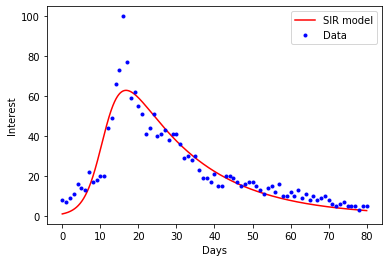
\includegraphics[width=0.8\linewidth]{cat}
    \label{fig:sfig1}
\end{subfigure}
\begin{subfigure}{.5\textwidth}
    \centering
    \caption{"baby yoda" starting 11/11/2019}
    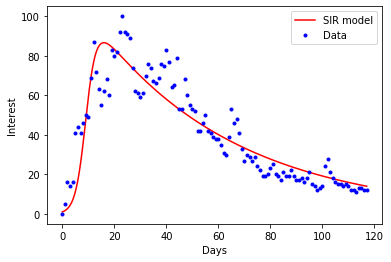
\includegraphics[width=0.8\linewidth]{yoda}
    \label{fig:sfig1}
\end{subfigure}
\caption{Plots of Google Trends data overlaid with a parameter optimized infection curve from the SIR model. The name of the term used in the Google Trends Search as well as the day of the first point are given.}
\label{fig:fig}
\end{figure}

All of the SIR model fits appear to accurately follow the Google Trends data for the most part. Fig. 1(a), (d), and (e) have peaks in the real-world data that rise significantly above the model. One of the key differences between these plots and the rest is that they gained popularity much faster, but, perhaps because of that, people lost interest in them more quickly resulting in a sharp peak that the SIR model cannot track fully. This cannot be confirmed without information on the absolute volume of searches for each meme, but it can be inferred by the sharpness of the peak. The initial growth period as well as the decline of the meme after the peak do fit the SIR model.

Another meme with a lot of points significantly far from the model is the "baby yoda" meme plotted in Fig 1(f). The general shape of the real-world data appears to fit the model, but there are days where the meme regains popularity significantly compared to where the model predicts its popularity should be. This is likely due to the fact that this particular meme is tied to a TV show called "The Mandalorian" which airs weekly and features the character of the "baby yoda" meme. As the SIR model does not account for people to become reinfected, it models the data poorly relative to the others. This problem of a meme having multiple popularity peaks is discussed in \cite{wang2011epidemiological}. They noted that in the real world, memes do not exist in isolation, so the constants of proportionality in the models must be time dependent in order to account for periodic events like a new episode of a TV show. So the SIR model fits well for the first peak, but it does not account for future peaks. However, the general downward trend in the popularity of the "baby yoda" meme is still captured by the standard SIR model used.

The "area 51" meme plotted in Fig 1(c) is the shortest lived meme, but it still demonstrates that an epidemics model can still be used to accurately describe the growth and decline of a meme that only lasts a month. The rest of the memes considered were fit well by the SIR model.

When fitting the model to the data, considering only $\beta$ and $\gamma$ as parameters with N fixed was insufficient for producing a representative curve for the Google Trends data. Looking at the values of N for each of the memes listed in Table 1 may be surprising as a population size in the hundreds seems unrealistically low. This may be due to the fact that the Google Trends data is not provided as the absolute number of searches. Google takes the raw data that they collect and normalize it in a way that obfuscates the meaning of N. Because the y axis of the graphs in Fig. 1 do not give the absolute number of infected, as is usually plotted in epidemiological contexts, N is not representative of the total number of people who engage with a particular meme. It is only a parameter that affects the shape of $I(t)$ while the least squares are being minimized.

These results support some of the conclusions reached in both \cite{bauckhage2011insights} and \cite{wang2011epidemiological}. Both papers found that epidemic models can be used to model the growth and decline of memes. However as a simpler model, the SIR model does not fit as well a the modified SIR model used in \cite{wang2011epidemiological} as the standard model does not accurately capture the peaks of a meme's popularity if the meme grows and declines very rapidly. This is the same conclusion that \cite{bauckhage2011insights} reached with the SIRS model. \cite{leskovec2007dynamics}, the paper discussing epidemic models in the context of viral marketing, did not find that SIR type models apply to viral marketing. Their results may be at odds with the ones in this paper depending on how similar viral marketing is compared to memes. However, more research needs to be done comparing the two before the results of \cite{leskovec2007dynamics} can be considered evidence against the viral spread of memes.

From these results idea that memes spread virally does not appear to be unfounded. While the SIR model used here is not perfect, the main problem being multiple peaks in popularity and extremely sharp peaks, different epidemiological models like SIS, MSEIR, and MSEIRS, described in \cite{hethcote2000mathematics} may provide better results. Studying these models and their respective parameters like $\beta$ and $\gamma$ provides insights on how a meme may behave which allows predictions on the popularity of memes over time. This enables those who wishes to take advantage of a meme for political or financial gain to gauge when a meme will peak and how well the meme continues to be popular based on that meme's initial growth period. This would allow marketing professionals to take advantage of a meme before the meme becomes stale allowing said professionals to connect with audiences in an effort to improve public relations and boost sales. If the spread of memes can be modeled by the spread of viruses, there is room to explore the meaning behind the proportionality constants used in the formulation of the SIR model (1). Increasing $\beta$ would increase the rate of infection allowing memes to spread quicker, and decreasing $\gamma$ would increase the amount of time a meme is relevant. This is the opposite of what epidemiologists try to do in order to limit the spread of disease, but often in the context of memes, the higher the number of infected the better. Finding ways of manipulating these parameters would further benefit marketing professionals.

While the data used in this paper appear to support the idea that memes spread virally, there are potential problems that need to be discussed. The most obvious of which being that the sample size of 6 memes may be insufficient to draw such a bold conclusion. This paper supports the claim that memes spread virally, and should be taken in the context of previous works like \cite{bauckhage2011insights} which examined 150 different memes. There may also be issues with time time range that the Google Trends data was taken. Most of the search terms used in Google Trends never fell to the interest level they were at before the creation of the first meme, and this may be an influencing factor on the shape of the infection curve. The 6 memes discussed in this paper had a single distinct peak, so memes with multiple clear peaks or where the popularity of a meme stayed consistent for a long period of time were not analyzed. \cite{bauckhage2011insights} and \cite{wang2011epidemiological} discusses these situations and have concluded that SIR type models can be describe flatter distributions, but not distributions with multiple peaks.

\section*{Conclusion}
Memes are a large part of today's internet with ample room for increased scientific research. Exploring the similarities between memes and infectious diseases is but a small yet intriguing part of that. This paper explores the claim that memes spread virally by examining how the well-known SIR model for disease epidemics fits data representing the popularity of 6 memes. These data was provided by Google Trends and were used to construct an infection curve of the meme. It was found that in general, memes do spread virally; however, the standard SIR model does not have the flexibility to describe memes that gain and lose popularity very quickly. As discussed in \cite{bauckhage2011insights} and \cite{wang2011epidemiological}, modifications to the SIR model or the use of a different epidemics model may provide better results in this situation. It was also found that the SIR model does not have the ability to model memes that have multiple peaks in popularity. In this case, either time dependent parameters, or a different model that considers periodic increases to the rate of infection, must be used instead.

Knowledge that the spread of memes can be described by epidemic models enables predictions on meme infection based on these models. Leveraging these models opens the door for marketing and campaigning with the aid of memes before the public loses interest. Further research into what influences the parameters of epidemic models like the transmission rate proportionality constant $\beta$ and the lost of interest proportionality constant $\gamma$ may lead to increased interest and longevity of the meme much like how epidemiologists try to reduce $\beta$ and increase $\gamma$ in order to limit the spread of real diseases.


\pagebreak
\bibliographystyle{apacite}
\bibliography{References}
\end{document}